\documentclass[11pt]{article}

\usepackage[margin=1.15in]{geometry}
\usepackage{amsmath}
\usepackage{amssymb}
\usepackage{graphicx}

% One symbol per object, as in notes/correlated_bias_prior_v2.
\newcommand{\Cov}{\mathsf{C}}
\newcommand{\T}{^{\mathsf{T}}}
\newcommand{\kmax}{k_{\rm max}}
\newcommand{\hMpc}{\,h/{\rm Mpc}}
% The unit of both counterterms.
\newcommand{\aunit}{\,h^{-2}\,{\rm Mpc}^2}
% The velocity dispersion of the Fingers-of-God blur.
\newcommand{\sv}{\sigma_v}
% The reference layout, as the reader-facing text names it.
\newcommand{\dcom}{$\Delta d_{\rm com} = 62$~Mpc}
% An underscore after which a long code name may break.
\newcommand{\us}{\_\allowbreak}
% The clause every caption that quotes k_max carries.
\newcommand{\kmaxclause}{$\kmax$ quoted at $z = 0$; each bin is cut at
  $\kmax/D(\bar{z}_i)$.}

\title{Does the counterterm $\alpha_2$ double count the
  Fingers-of-God dispersions?}
\date{November 2026}
\author{}

\begin{document}

\begin{center}
  {\LARGE Does the counterterm $\alpha_2$ double count\\[0.3em]
    the Fingers-of-God dispersions?\par}
  \vspace{0.6em}
  {\large The redshift-space counterterm against the sampled velocity
    dispersions $\sv$,\\ template by template and in the posterior\par}
  \vspace{1em}
  {\large November 2026\par}
\end{center}
\vspace{1em}

\section{Summary}
\label{sec:summary}

\paragraph{The question.}
The forecast's one-loop model carries two descriptions of nonlinear
velocities along the line of sight.  One is the Fingers-of-God blur:
each bin's redshift distribution is convolved with a Gaussian whose
width is set by a velocity dispersion $\sv$, one per dispersion group,
sampled under a Gaussian prior.  The other is the line-of-sight
counterterm $\alpha_2$ of the DESI 2024 full-shape
convention~\cite{Maus2024},
\begin{equation}
  P_{\rm CT}(k, \mu) \;=\; \bigl(b_1 + f\mu^2\bigr)\,
  f\,\alpha_2\,\mu^2 k^2\,P_{\rm lin}(k) ,
  \label{eq:alpha2}
\end{equation}
with $k$ the comoving wavenumber, $\mu$ the cosine of the angle to the
line of sight, $b_1$ the bin's linear galaxy bias, $f = d\ln D/d\ln a$
the linear growth rate ($D$ the linear growth factor, $a$ the scale
factor), $P_{\rm lin}$ the linear matter power spectrum, and
$\alpha_2$ in $h^{-2}\,{\rm Mpc}^2$, one value per group plus a free
tilt in redshift in model B + tilts.  The leading effect of the blur
on the power spectrum is a damping $-\sigma_\chi^2 k_\parallel^2$ with
$k_\parallel = k\mu$ and $\sigma_\chi = (1 + z)\,\sv/H(z)$ the
dispersion in comoving distance: the same $k_\parallel^2$ shape as
Eq.~\eqref{eq:alpha2} (Section~\ref{sec:why}).  So the question is
whether the forecast pays twice for one effect: is $\alpha_2$
degenerate with the $\sv$ already in the model?

\paragraph{The answer.}
\begin{enumerate}
  \item \textbf{At the template level, yes.}  On every layout and at
    every cut, combinations of the seven $\sv$ templates reproduce
    $95.8$--$100\%$ of each $\alpha_2$ group template's information in
    the $\Cov^{-1}$ metric ($\Cov$ the band-power covariance), with
    medians $99.3$--$99.9\%$; the two templates are mirror images, so
    a positive $\alpha_2$ looks like a smaller $\sv$
    (Figure~\ref{fig:templates}).  Only the $\alpha_2$ tilt columns
    are substantially new.
  \item \textbf{In the posterior, the $\sv$ priors break the
    degeneracy at small cuts but not at large ones.}  In the paper
    model (model B + tilts on the pessimistic linear-bias prior) the
    largest correlation between an $\alpha_2$ parameter and a $\sv$
    grows, on the thin layouts, from $|\rho| = 0.39$--$0.46$ at
    $\kmax = 0.075\hMpc$ to $0.81$--$0.88$ at $0.2$
    (Figure~\ref{fig:kmax}).
  \item \textbf{What $\alpha_2$ costs.}  Fixing $\alpha_2$ and its
    tilts at zero raises ${\rm FoM}(w_0, w_a)$ of the paper model by a
    factor of $2.4$--$2.7$ at $0.075$ and $1.16$--$1.25$ at $0.2$ on
    the thin layouts; ${\rm FoM}(\Omega_m, 10^9 A_s)$ moves the same
    way.  The gain comes entirely from the $\sv$ priors: with flat
    $\sv$ priors, fixing $\alpha_2$ returns $0.83$--$1.01$ of the
    paper model's FoM at every cut from $0.075$ on.
  \item \textbf{What dropping $\alpha_2$ risks.}  If the truth holds a
    DESI-prior-sized $\alpha_2 = 12.5\aunit$ in every group, a fit
    without $\alpha_2$ (model A + tilts) is shifted in $(w_0, w_a)$,
    and $\sv$ on its priors absorbs almost none of it: the shift falls
    by $4\%$ and $17\%$ at $0.075$ and by $35\%$ and $41\%$ at $0.2$
    on the two thin layouts.  With flat $\sv$ priors those shifts fall
    by $88$--$97\%$.  The wide layouts barely react either way.
  \item \textbf{A wider $\sv$ prior trades the gain for the
    absorption.}  Multiplying all seven $\sv$ prior widths by a common
    factor $s$, the fit without $\alpha_2$ absorbs the
    $12.5\aunit$ truth (every shift below $\sigma/3$) at $s = 1.84$
    and $1$ at $\kmax = 0.075\hMpc$ on the thin layouts, where it
    still keeps $2.1$ and $2.8$ times the paper model's FoM; at
    $0.1$--$0.2$ it absorbs only at $s = 3.6$--$6.0$, where the FoM
    ratio is $0.96$--$1.22$ and the gain is gone
    (Figure~\ref{fig:sigvwidth}).  Widening one sample's dispersions
    alone never suffices at $0.1$ and above.
\end{enumerate}
Here $w_0$ and $w_a$ parameterize the dark-energy equation of state
$w(a) = w_0 + w_a(1 - a)$; $\Omega_m$ is the matter density today in
units of the critical density; $A_s$ is the amplitude of the primordial
curvature power spectrum, sampled as $10^9 A_s$; and
${\rm FoM}(w_0, w_a) = [\det{\rm Cov}(w_0, w_a)]^{-1/2}$ is the inverse
area of the marginalized $(w_0, w_a)$ ellipse, likewise
${\rm FoM}(\Omega_m, 10^9 A_s)$.  In short: one $k_\parallel^2$ effect,
counted twice at the template level; the posterior keeps the two apart
only as long as the $\sv$ priors do, and the whole dark-energy gain of
dropping $\alpha_2$ is exactly as strong as those priors.  Whether to
keep both, and on what basis for the $\sv$ priors, is an open decision
(appendix ``Open issues'').

\paragraph{The setup.}
The data are the DESI angular clustering band powers $C_\ell^{gg}$
alone, computed without the Limber approximation, on four bin layouts:
\dcom{} (equal comoving width) and $\Delta z = 0.02$, $0.05$ and $0.2$
(fixed redshift width); the first two are the thin layouts.  The scan
runs over $\kmax = 0.05$ to $0.2\hMpc$, each the $z = 0$ value of a
per-bin cut at $\kmax/D(\bar{z}_i)$, with $\bar{z}_i$ the mean redshift
of bin $i$.  Every number and figure of this note comes from the final
section of \texttt{EXAMPLE\us EVALUATE\us FISHER\us MODEL\us B.ipynb};
the per-cut values are in the two figure folders'
\texttt{data.json}.

\begin{figure}[p]
  \centering
  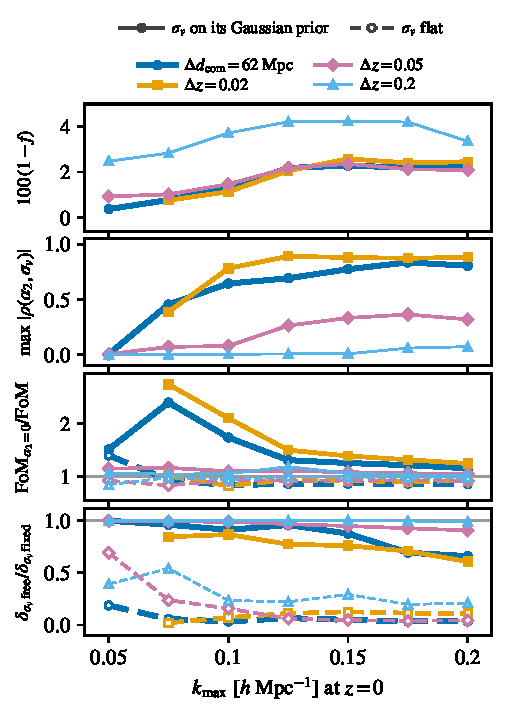
\includegraphics[width=3.5in]{plots/fog_degeneracy_kmax/fog_degeneracy_kmax.pdf}
  \caption{How far the counterterm $\alpha_2$ and the Fingers-of-God
    dispersions $\sv$ describe the same band powers, against the scale
    cut, per layout (color, line width and marker; legend).  Top
    panel: $100\,(1 - f)$, the share of an $\alpha_2$ group template's
    information in the $\Cov^{-1}$ metric that no combination of the
    seven $\sv$ templates reproduces, for the group where that share
    is largest; this panel is built from the templates and the
    covariance alone and does not depend on any prior.  Second panel:
    the largest $|\rho|$ between an $\alpha_2$ parameter and a $\sv$
    in the posterior of the paper model, model B + tilts on the
    pessimistic linear-bias prior.  Third panel:
    ${\rm FoM}_{\alpha_2 = 0}/{\rm FoM}$, the ${\rm FoM}(w_0, w_a)$
    with $\alpha_2$ and its tilts fixed at zero over the paper
    model's, with $\sv$ on its Gaussian priors (solid, filled markers)
    or flat (dashed, open markers).  Bottom panel:
    $\delta_{\sv\,{\rm free}}/\delta_{\sv\,{\rm fixed}}$, with
    $\delta$ the $(w_0, w_a)$ shift of model A + tilts, which has no
    $\alpha_2$, fitted to a truth with $\alpha_2 = 12.5\aunit$ in
    every group: the shift with $\sv$ free over the shift with $\sv$
    fixed at its fiducial, with the same two line styles.
    Gray: one.  $\Delta z = 0.02$ keeps no band at $0.05\hMpc$.
    \kmaxclause}
  \label{fig:kmax}
\end{figure}

\section{Why the question is natural}
\label{sec:why}

\paragraph{Redshift is blurred distance.}
The forecast places each galaxy at its measured redshift.  Inside
groups and clusters, galaxies orbit with random speeds of several
hundred km/s, so a galaxy's measured redshift carries a Doppler shift
on top of its distance: in a redshift map a cluster stretches into a
finger pointing at the observer, the Fingers of
God~\cite{Jackson1972}.  A line-of-sight velocity $v$ at redshift $z$
displaces the galaxy by
\begin{equation}
  \delta\chi \;=\; \frac{(1 + z)\,v}{H(z)} ,
  \label{eq:conversion}
\end{equation}
with $\chi$ the comoving distance and $H(z)$ the expansion rate.  A
dispersion $\sv$ of these velocities blurs distances by
$\sigma_\chi = (1 + z)\,\sv/H(z)$: for the groups here, $5$--$6$~Mpc,
about $4\,h^{-1}$Mpc (\texttt{notes/cross\us correlations}, which
derives the convolution and its sizes).

\paragraph{Blurring the window equals blurring the field.}
The likelihood implements the blur by convolving each bin's redshift
distribution $n_i(z)$ with a Gaussian of width
$(1 + \bar{z}_i)\,\sv/c$ in redshift~\cite{GrasshornGebhardt2020}.
That window-side convolution is the same operation as damping the
three-dimensional field, as long as the velocities are a random
scatter uncorrelated with the density.  Write the observed galaxy
field as the true one with each galaxy moved by $\delta\chi$ drawn
from a distribution $p$: along one line of sight,
$\delta_g^{\rm obs}(\chi_{\rm obs}) = \int d\chi\,
p(\chi_{\rm obs} - \chi)\,\delta_g(\chi)$.  A bin's map integrates the
observed field over its radial window $W_i$:
\begin{align}
  \int d\chi_{\rm obs}\, W_i(\chi_{\rm obs})\,
  \delta_g^{\rm obs}(\chi_{\rm obs})
  \;&=\; \int d\chi\,\Bigl[\int d\chi_{\rm obs}\,
  W_i(\chi_{\rm obs})\, p(\chi_{\rm obs} - \chi)\Bigr]\,
  \delta_g(\chi)
  \nonumber\\
  \;&=\; \int d\chi\,\bigl(W_i \!*\! p\bigr)(\chi)\,
  \delta_g(\chi) :
  \label{eq:swap}
\end{align}
swapping the order of integration moves the convolution from the field
onto the window.  Blurring every bin's $n(z)$ and keeping the true
field is therefore the same map as keeping sharp bins and blurring the
field, which is how the likelihood's $\sv$ reach the spectra.

\paragraph{The damping and its leading order.}
On the field side, a convolution along the line of sight multiplies
each Fourier mode by the distribution's transform: for a Gaussian $p$
of width $\sigma_\chi$, the density picks up
$\exp(-k_\parallel^2\sigma_\chi^2/2)$ and the power spectrum
$\exp(-k_\parallel^2\sigma_\chi^2)$, with $k_\parallel = k\mu$ the
line-of-sight wavenumber.  Applied to the linear redshift-space
(Kaiser~\cite{Kaiser1987}) power, to leading order in
$k_\parallel^2\sigma_\chi^2$,
\begin{equation}
  \bigl(b_1 + f\mu^2\bigr)^2 P_{\rm lin}\,
  e^{-k_\parallel^2\sigma_\chi^2}
  \;\simeq\;
  \bigl(b_1 + f\mu^2\bigr)^2 P_{\rm lin}
  \;-\; \sigma_\chi^2\, k_\parallel^2\,
  \bigl(b_1 + f\mu^2\bigr)^2 P_{\rm lin} .
  \label{eq:damping}
\end{equation}
The counterterm, Eq.~\eqref{eq:alpha2}, is
$f\,\alpha_2\,k_\parallel^2\,(b_1 + f\mu^2)\,P_{\rm lin}$.  Both are
$k_\parallel^2$ times the linear power; their $\mu$ structures differ
by exactly one factor of $(b_1 + f\mu^2)$, and a band power averages
much of that difference away.  The signs are opposite where both
amplitudes are positive: a positive $\alpha_2$ raises the spectrum
where a larger $\sv$ lowers it, so a positive $\alpha_2$ looks like a
\emph{smaller} $\sv$.  The sizes are comparable too:
$\sigma_\chi \approx 4\,h^{-1}$Mpc gives
$\sigma_\chi^2 \approx 16\aunit$, the order of the DESI prior width
$12.5\aunit$ of $\alpha_2$ at $\kmax = 0.2\hMpc$.

\paragraph{Why both exist.}
In a three-dimensional full-shape analysis there is no radial window
to convolve, so there is no sampled $\sv$: the counterterm $\alpha_2$
is that analysis's effective description of small-scale velocities,
Fingers of God included~\cite{Maus2024,DESI2024V}.  This forecast
works on projected spectra, where the window-side convolution is
natural and $\sv$ already carries the effect; $\alpha_2$ was added
with the rest of the DESI counterterm set.  A setup with $\alpha_0$
only -- the density counterterm, which multiplies $k^2 P_{\rm mm}$
with no $\mu$ -- is the natural alternative, and this note measures
what each choice costs.

\paragraph{The seven dispersions and their priors.}
Each bin's $\sv$ is its dispersion group's value
(Table~\ref{tab:sigv}): the measured dispersion curve of the source
forecast's simulated galaxies steps inside BGS, so BGS takes two
values, split at $\bar{z} = 0.255$, giving seven dispersion groups for
six bias groups.  Each prior is a Gaussian centred on the measured
value, five times as wide as that measurement's per-bin error bar, and
truncated at zero; the defaults and priors live in
\texttt{likelihood/params\us desi*.yaml} (the \texttt{DESI\us SIGV}
parameters, one sampled value per group), and their provenance is the
section ``Where the velocity dispersions come from'' of
\texttt{notes/cross\us correlations}.  The same seven values and
widths serve every layout.

\begin{table}[ht]
  \centering
  \begin{tabular}{lcc}
    \hline
    dispersion group & $\sv$ [km/s] & prior width [km/s] \\
    \hline
    BGS, $\bar{z}_i < 0.255$ & $371$ & $145$ \\
    BGS, $\bar{z}_i \ge 0.255$ & $358$ & $105$ \\
    LRG1 & $357$ & $70$ \\
    LRG2 & $348$ & $50$ \\
    LRG3 & $343$ & $50$ \\
    ELG1 & $304$ & $40$ \\
    ELG2 & $289$ & $30$ \\
    \hline
  \end{tabular}
  \caption{The fiducial velocity dispersion of each group and the
    width $\Delta\sigma_{v,g}$ of its Gaussian prior.}
  \label{tab:sigv}
\end{table}

\section{Templates, and how to measure redundancy}
\label{sec:method}

\paragraph{A parameter's template.}
A parameter $p$'s template is the derivative of the data vector,
$\partial C_\ell/\partial p$ over every kept band of every spectrum.
To first order it is the fingerprint $p$ leaves on the data: the fit
can distinguish two parameters only as far as their templates differ.
Each parameter is measured in units of its prior width $\Delta_p$
(written $\Delta$, never $\sigma$, since $\sv$ is itself a
dispersion): here $\Delta\alpha_2 = 0.5/\kmax^2$, the model B prior
width, quoted at $\kmax = 0.2\hMpc$ where it is $12.5\aunit$, and
$\Delta\sigma_{v,g}$ each dispersion group's prior width
(Table~\ref{tab:sigv}).  Divided by each band's error
$\sigma_\ell = \sqrt{\Cov_{ii}}$, the scaled template
$\sigma_\ell^{-1}\,\partial C_\ell/\partial(p/\Delta_p)$ reads
directly as how many error bars the parameter can move each band while
staying within its prior; Figure~\ref{fig:templates} draws the
templates this way, following Fig.~1 of Obied et
al.~\cite{Obied2017}.  The $\alpha_2$ templates here are group
templates: the response to the group's value, all bins of the group
moving together (and, for the tilts, moving along a straight line in
redshift).

\paragraph{The leftover, measured in the data's own error bars.}
Can an $\alpha_2$ group template be rebuilt as a weighted sum of the
seven $\sv$ templates?  The leftover of the best weights $c_g$ is
\begin{equation}
  r_\ell \;=\; \frac{\partial C_\ell}{\partial(\alpha_2/\Delta\alpha_2)}
  \;-\; \sum_{g} c_g\,
  \frac{\partial C_\ell}{\partial(\sigma_{v,g}/\Delta\sigma_{v,g})} ,
  \label{eq:leftover}
\end{equation}
the sum running over the seven dispersion groups.  It should not be
measured band by band: a mismatch of $0.1\sigma_\ell$ on a precise
band is visible where the same mismatch on a noisy band is not.  The
natural norm is the data's own, $r\T \Cov^{-1} r$ with $r$ the vector
of the $r_\ell$, the $\chi^2$ the leftover would contribute, and the
weights $c_g$ minimize it.  Writing $a$ for the scaled $\alpha_2$
template, the first term of Eq.~\eqref{eq:leftover}, the redundancy
fraction is the share of the template's information that the $\sv$
templates reproduce,
\begin{equation}
  f \;=\; 1 \;-\; \frac{\min_c\, r\T\, \Cov^{-1}\, r}
  {a\T\, \Cov^{-1}\, a} .
  \label{eq:fdef}
\end{equation}
$f = 1$ means the data cannot tell $\alpha_2$ from that combination of
dispersions at all.  (The letter $f$ follows the figure axis; the
growth rate is written $f$ only inside
Eqs.~\eqref{eq:alpha2} and~\eqref{eq:damping}.)

\paragraph{A three-band toy.}
Take three bands with unit error bars and two templates,
$a = (1, 2, 3)$ and $s = (2, 4, 6)$.  Then $a = s/2$ exactly: the
leftover is zero and $f = 1$; whatever signal $a$ could produce, $s/2$
produces identically, and the data cannot separate the two parameters.
Now take $s = (2, 4, 5)$, which differs from $2a$ only on the third
band.  The best single weight is $c = 5/9$, the leftover is
$r = (-1, -2, 2)/9$ with $r\T r = 1/9$, and
$f = 1 - (1/9)/14 = 0.992$.  Whether that mismatch matters is decided
by the third band's error bar.  If the third band is noisy, the fit
matches the first two bands almost exactly and hides the whole
mismatch inside the third band's error: the leftover $\chi^2$ falls
toward zero and $f \to 1$.  If the third band is precise, the fit is
pinned there ($c \to 3/5$) and the mismatch is pushed onto the first
two bands as a visible leftover.  Either way, a mismatch is only as
detectable as the error bars of the bands where it must appear --
which is what the $\Cov^{-1}$ weighting in Eq.~\eqref{eq:fdef} counts.

\paragraph{One parameter against one: $f = \rho^2$.}
With one $\alpha_2$ amplitude, one $\sv$ and nothing else free
(templates $a$ and $s$), the
two-parameter Fisher matrix is built from $a\T\Cov^{-1}a$,
$a\T\Cov^{-1}s$ and $s\T\Cov^{-1}s$, and the correlation of its
inverse is $\rho = -\,a\T\Cov^{-1}s\,/\sqrt{(a\T\Cov^{-1}a)
(s\T\Cov^{-1}s)}$, so $\rho^2 = f$.  Mirror-image templates
($a\T\Cov^{-1}s < 0$) give a \emph{positive} posterior correlation:
the direction the data cannot see has $\alpha_2$ and $\sv$ rising
together, each undoing the other's change of the spectra.  The
posterior correlation of the full model is a different number from
$f$: it marginalizes every other parameter -- cosmology, biases, the
other counterterms -- which can soak up part of either template, and
it includes the priors, which hold parameters the data would let
drift.  That is why $f$ can sit at $0.99$ while $|\rho|$ ranges from
$0.003$ to $0.90$ across cuts and layouts.

\paragraph{Many against many: canonical correlations.}
For the full sets -- six $\alpha_2$ group columns (plus tilts) against
seven $\sv$ columns -- the squared canonical correlations generalize
$\rho^2$: they are the cosines of the principal angles between the two
template subspaces in the $\Cov^{-1}$ metric, the per-direction
version of Eq.~\eqref{eq:fdef}.

\section{Results}
\label{sec:results}

\paragraph{The templates are mirror images.}
Figure~\ref{fig:templates} draws the $\alpha_2$ and $\sv$ templates of
three \dcom{} spectra, each scaled by its prior width.  The two
templates track each other band by band with opposite signs, at a few
tenths of $\sigma_\ell$ per band.  The bottom row is the leftover
$r_\ell$ of Eq.~\eqref{eq:leftover}: after the best combination of the
seven $\sv$ templates, fitted over the whole data vector,
$|r_\ell|/\sigma_\ell$ stays below $0.04$ per band in the BGS panel
and below $0.013$ in the LRG panels at the $0.2\hMpc$ cut, and below
$0.004$ everywhere at $0.075$: templates of a few tenths of an error
bar cancel to a few thousandths.

\begin{figure}[t]
  \centering
  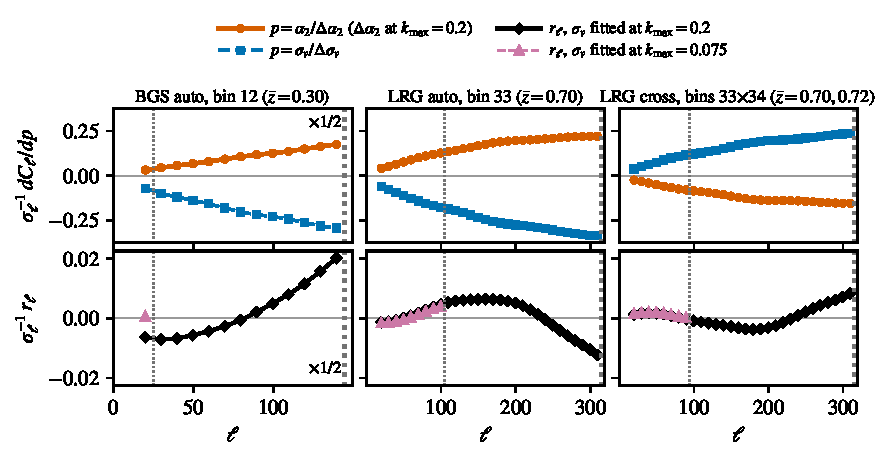
\includegraphics[width=\linewidth]{plots/fog_templates/fog_templates.pdf}
  \caption{The $\alpha_2$ and $\sv$ templates of three
    \dcom{} spectra -- a BGS auto spectrum ($\bar{z} = 0.28$), an LRG
    auto spectrum ($\bar{z} = 0.70$) and that bin's cross spectrum
    with the next LRG bin -- in units of each band's error
    $\sigma_\ell = \sqrt{\Cov_{ii}}$, on the bands the shipped mask
    keeps; the BGS column is divided by the round factor written in
    its panels, and each row shares one $y$ axis.  Top row: the scaled
    templates $\sigma_\ell^{-1}\,\partial C_\ell/\partial p$, each
    parameter in units of its prior width: $p = \alpha_2/\Delta\alpha_2$
    of the bin's group, with $\Delta\alpha_2$ the prior width at
    $\kmax = 0.2\hMpc$ (vermillion solid, circles), and
    $p = \sv/\Delta\sv$ of the bin's dispersion (blue dashed,
    squares).  Bottom row: $\sigma_\ell^{-1} r_\ell$, the leftover of
    the $\alpha_2$ template after its best combination of the seven
    $\sv$ templates, Eq.~\eqref{eq:leftover}, fitted over the whole
    data vector in the $\Cov^{-1}$ metric on the bands a cut keeps and
    drawn on those bands, for $\kmax = 0.2$ (black, diamonds) and
    $0.075\hMpc$ (pink dashed, triangles).  Dotted vertical lines:
    where the shown spectrum's kept bands end at $0.075$ (thin) and at
    $0.2$ (thick).
    \kmaxclause}
  \label{fig:templates}
\end{figure}

\paragraph{The redundancy against the cut.}
Over all four layouts and every cut of the scan, $f$ of the six
$\alpha_2$ group columns lies between $0.958$ and $1.000$, with
per-cut medians of $0.993$--$0.999$; the squared canonical
correlations of the six-column $\alpha_2$ set with the seven-column
$\sv$ set lie in the same range, $0.958$--$1.000$.  The top panel of
Figure~\ref{fig:kmax} draws $100\,(1 - f)$ for the least redundant
group: even there, at most $4.3\%$ of the template's information is
new.  The $\alpha_2$ \emph{tilt} columns are much less redundant --
their per-cut medians lie between $0.03$ and $0.24$ at every cut
except the smallest cut on \dcom{}, where only three tilt columns keep
any band -- because a straight line in redshift across a group is a
shape no combination of seven group-constant dispersions reproduces.
At the template level, then, the $\alpha_2$ group values duplicate
information the $\sv$ already carry; the tilts are the genuinely new
freedom.

\paragraph{The posterior of the paper model.}
The second panel of Figure~\ref{fig:kmax} shows the largest
$|\rho(\alpha_2, \sv)|$ in the paper model's posterior.  On the thin
layouts it grows from $0.46$ (\dcom{}) and $0.39$ ($\Delta z = 0.02$)
at $\kmax = 0.075\hMpc$ to $0.81$ and $0.88$ at $0.2$, peaking at
$0.84$ and $0.90$ at intermediate cuts; on $\Delta z = 0.05$ it stays
at $0.08$--$0.37$, and on $\Delta z = 0.2$ below $0.10$.  Wherever the
correlation is appreciable, the pair is LRG3's $\alpha_2$ with LRG3's
own dispersion, and its sign is positive, as mirror-image templates
give (Section~\ref{sec:method}).  The correlations stay below one
because the $\sv$ priors hold their end of the degenerate direction:
with $\alpha_2$ free, every $\sv$ posterior keeps $0.60$--$1.00$ of
its prior width, so the dispersions stay prior-dominated while
$\alpha_2$ takes the $k_\parallel^2$ information.  With $\alpha_2$ and
its tilts fixed, the data begin to measure the dispersions: on the
thin layouts the best-measured $\sv$ tightens to $0.25$--$0.74$ of its
prior width at cuts of $0.075$ and above.

\paragraph{What $\alpha_2$ costs.}
The third panel of Figure~\ref{fig:kmax} draws
${\rm FoM}_{\alpha_2 = 0}/{\rm FoM}$: the paper model with $\alpha_2$
and its tilts fixed at zero, over the paper model.  On the
thin layouts the fixed fit has $2.41$ and $2.70$ times the
${\rm FoM}(w_0, w_a)$ at $\kmax = 0.075\hMpc$, $1.73$ and $2.10$ at
$0.1$, and $1.16$ and $1.25$ at $0.2$; ${\rm FoM}(\Omega_m, 10^9 A_s)$
gains similar factors ($2.27$ and $2.19$ at $0.075$, $1.18$ and $1.25$
at $0.2$).  On $\Delta z = 0.05$ the gain is $1.05$--$1.17$, and on
$\Delta z = 0.2$ at most $1.07$ at every cut except $0.125$, where it
reaches $1.19$.  The dashed curves isolate where the gain comes from:
with the $\sv$ priors removed (flat), fixing $\alpha_2$ returns
$0.83$--$1.01$ of the paper model's FoM at every cut from $0.075$ on
-- no gain at all.  Fixing $\alpha_2$ therefore does not add
information of its own; it hands the $k_\parallel^2$ direction to the
dispersions, and the constraint the fixed fit gains is exactly the
constraint the $\sv$ priors supply.

\paragraph{What dropping $\alpha_2$ risks.}
The absorption test fits model A + tilts, which has no $\alpha_2$, to
a truth with $\alpha_2 = 12.5\aunit$ in every group -- the DESI prior
width at $\kmax = 0.2\hMpc$.  If $\sv$ could stand in for $\alpha_2$
in practice, freeing it would absorb the shift.  It barely does: with
$\sv$ on its Gaussian priors, the $(w_0, w_a)$ shift falls from the
fixed-$\sv$ value by $4\%$ at $0.075$ ($0.335 \to 0.322$ ellipse
units) and $35\%$ at $0.2$ ($1.65 \to 1.07$) on \dcom{}, and by $17\%$
($0.305 \to 0.254$) and $41\%$ ($2.60 \to 1.54$) on $\Delta z = 0.02$;
on $\Delta z = 0.05$ by at most $9\%$, and on $\Delta z = 0.2$ the
shift never exceeds $0.016\sigma$ to begin with.  With flat $\sv$
priors the same shifts, at cuts of $0.075$ and above, fall by
$88$--$97\%$ (bottom panel of
Figure~\ref{fig:kmax}): the dispersions \emph{can} mimic the
counterterm, but only by moving far outside their priors.  Fitting the
$\alpha_2 = 12.5\aunit$ truth with the $\sv$ templates alone makes
this concrete: on \dcom{} at $0.2$ the truth carries
$\Delta\chi^2 = 162$, of which free dispersions leave $1.6$ -- but the
mimicking shift is $-2.5$ prior widths ($-75$~km/s, always the ELG2
dispersion, whose prior is tightest), and with the Gaussian priors the
total left, data residual plus prior penalty, is $14$.  Across the
thin layouts at cuts of $0.075$ and above, the mimicking shift is
$1.9$--$2.6$ prior widths ($57$--$78$~km/s).  The shifts scale
linearly with the truth: a truth at one model B prior width
($0.5/\kmax^2$, $88.9\aunit$ at $0.075$) gives $7.1$ times the
$12.5\aunit$ shifts there.

\section{How wide must the $\sv$ priors be?}
\label{sec:width}

\paragraph{The knob.}
The absorption test leaves a natural follow-up question: if $\sv$
keeps a Gaussian prior, how wide must that prior be for the
dispersions to absorb a DESI-size $\alpha_2$?  The two preceding
results frame the answer before any scan.  Mimicking
$\alpha_2 = 12.5\aunit$ costs the dispersions $1.9$--$2.6$ prior
widths, so widening the priors by a factor of a few makes that move
cheap and the shift disappears.  But the FoM gain of dropping
$\alpha_2$ comes entirely from those same priors, so the same widening
surrenders the gain.  A single knob -- a common factor $s$ on all
seven prior widths of Table~\ref{tab:sigv} -- therefore slides the fit
between two ends: at $s = 1$ the full gain and almost no absorption,
with flat priors the full absorption and no gain.  The scan locates
where between the two ends each layout and cut sits.

\paragraph{The scan.}
The fit is the one of the absorption test -- model A + tilts on the
pessimistic linear-bias prior, which carries $\alpha_0$ but no
$\alpha_2$: the $\alpha_0$-only setup of Section~\ref{sec:why} --
fitted to the truth $\alpha_2 = 12.5\aunit$ in every group, with all
seven $\sv$ prior widths multiplied by
$s \in \{1, 1.5, 2, 3, 5, 10\}$ and flat.  Each $s$ is scored by
$\delta_{\max}$, the largest of the $(w_0, w_a)$ shift in its ellipse
and the $\Omega_m$ and $A_s$ shifts in their own $\sigma$, and by
${\rm FoM}_{\alpha_0\,{\rm only}}/{\rm FoM}$, that fit's
${\rm FoM}(w_0, w_a)$ over the paper model's at $s = 1$.  The passing
$s$ is the smallest $s$ with every shift below $\sigma/3$,
interpolated linearly in $\log s$ between the scanned values.
Figure~\ref{fig:sigvwidth} draws the scan; every cut, the per-shift
values and the one-sample variants below are in that folder's
\texttt{data.json}.

\paragraph{At $\kmax = 0.075\hMpc$ the default priors almost
suffice.}
\dcom{} passes at $s = 1.84$, keeping $2.13$ times the paper model's
FoM; $\Delta z = 0.02$ passes at $s = 1$, keeping $2.77$.
$\Delta z = 0.05$ passes at $s = 1$ at every cut up to $0.15$
(FoM ratios $1.12$--$1.23$) and needs $s \approx 2.9$ at
$0.175$--$0.2$, where the ratio is $1.02$--$1.03$; $\Delta z = 0.2$
passes at $s = 1$ everywhere ($1.05$--$1.25$).

\paragraph{At $0.1$--$0.2$ on the thin layouts the two options
converge.}
There the passing factor is $s = 3.56$--$3.83$ on \dcom{} and
$4.83$--$5.99$ on $\Delta z = 0.02$: ELG2's $30$~km/s prior becomes
about $110$--$180$~km/s, a third to more than half of its fiducial
dispersion.  At those widths the FoM ratio is $0.96$--$1.22$: the
widened $\alpha_0$-only fit and the paper model constrain dark energy
essentially equally, and the gain that motivated dropping $\alpha_2$
is gone.

\paragraph{One sample's dispersions alone do not absorb it.}
The truth holds $\alpha_2$ in every group, so the mimicking must too.
Widening only the three LRG dispersions fails wherever $s = 1$ does
not already pass: on \dcom{} at $0.2$, $\delta_{\max}$ falls only from
$1.16$ to $1.12$ even with the LRG priors flat.  Widening only the two
ELG dispersions passes on \dcom{} at $0.075$ ($s = 2.94$, ratio
$2.24$) and on $\Delta z = 0.05$ at $0.175$--$0.2$, but fails on the
thin layouts at $0.1$ and above.  Absorbing $\alpha_2$ needs all the
dispersions widened together.

\begin{figure}[t]
  \centering
  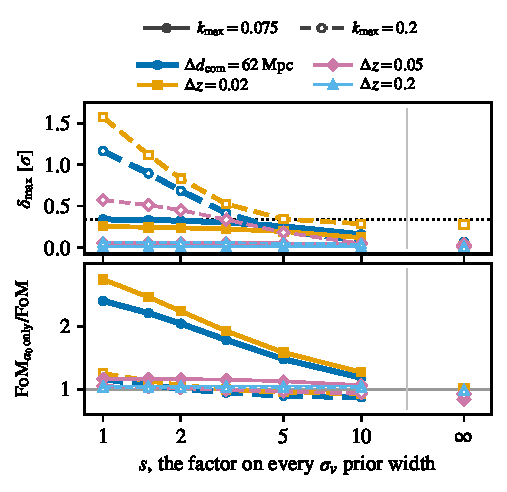
\includegraphics[width=3.5in]{plots/fog_sigv_width/fog_sigv_width.pdf}
  \caption{The $\sv$ prior-width scan: the $\alpha_0$-only fit (model
    A + tilts on the pessimistic linear-bias prior) fitted to a truth
    with $\alpha_2 = 12.5\aunit$ in every group, against $s$, the
    common factor on all seven $\sv$ prior widths (log axis; the
    flat-$\sv$ points sit at the right edge, past the gap), per layout
    (color, line width and marker; legend) at $\kmax = 0.075\hMpc$
    (solid, filled markers) and $0.2$ (dashed, open markers).  Top
    panel: $\delta_{\max}$, the largest of the $(w_0, w_a)$ shift in
    its ellipse and the $\Omega_m$ and $A_s$ shifts in their own
    $\sigma$; dotted: $\sigma/3$.  Bottom panel:
    ${\rm FoM}_{\alpha_0\,{\rm only}}/{\rm FoM}$, that fit's
    ${\rm FoM}(w_0, w_a)$ over the paper model's, model B + tilts with
    $\alpha_2$ free and $\sv$ at $s = 1$; gray: one.  \kmaxclause}
  \label{fig:sigvwidth}
\end{figure}

\section{What this means}
\label{sec:meaning}

At the template level, $\alpha_2$ and the sampled $\sv$ carry the same
$k_\parallel^2$ information: in that sense the model double counts one
physical effect, and the $\alpha_2$ group values add almost no
template direction the dispersions do not already span.  Only the
$\alpha_2$ tilts are new.

In the posterior, the Gaussian $\sv$ priors break the degeneracy.
They are tight enough (10--40\% of the fiducial dispersions) that the
dispersions cannot wander along the degenerate direction, so the joint
fit stays well conditioned at every cut, with the largest
$\alpha_2$--$\sv$ correlation reaching $0.9$ only at the largest cuts
on the thin layouts.

Keeping both parameters has a definite division of labor: $\alpha_2$,
with its wide prior, takes the $k_\parallel^2$ information, and the
dispersions fall back to their priors ($0.60$--$1.00$ of the prior
width with $\alpha_2$ free).  The data then constrain nonlinear
velocities only as far as the $\alpha_2$ prior allows, and the $\sv$
priors contribute almost nothing to the FoM.

Dropping $\alpha_2$ gains a factor of $2.4$--$2.7$ in
${\rm FoM}(w_0, w_a)$ at $\kmax = 0.075\hMpc$ and $1.16$--$1.25$ at
$0.2$ on the thin layouts -- a gain that is exactly as good as the
$\sv$ priors, since it vanishes when those priors are removed.  The
same move carries the bias risk of the absorption test: if a
DESI-prior-sized $\alpha_2$ is present in the truth, a fit without
$\alpha_2$ is shifted by up to $0.34$ ellipse units at $0.075$ and
$1.6$--$2.6$ at $0.2$ on the thin layouts, and the dispersions on
their priors absorb at most $4$--$41\%$ of it.  The wide layouts
barely care either way: their gains are at most $\sim\!20\%$ and their
shifts at most $0.43\sigma$ ($\Delta z = 0.05$ at $0.2$).

These are the trade-offs as measured; whether the forecast keeps
$\alpha_2$, drops it in favor of the dispersions, or moves to a setup
with $\alpha_0$ only is not decided in this note (appendix ``Open
issues'').

\appendix

\section{Method and checks}
\label{app:method}

\paragraph{Machinery.}
Everything runs on the model B notebook's final section
(Section~\ref{sec:summary} names the file): the
final-tier derivative caches of that notebook (five-point
stencils; the $\alpha_2$ columns are exact one-difference templates,
since the term is linear in its amplitude), the Gaussian band-power
covariance restricted to the bands each cut keeps, and the notebook's
Fisher systems $F = \mathsf{D}\T\Cov^{-1}\mathsf{D} + F_{\rm priors}$,
with $\mathsf{D}$ the derivative matrix and $F_{\rm priors}$ the
Gaussian priors of the paper model (the pessimistic linear-bias prior,
the one-loop offset and counterterm priors, and the $\sv$ priors of
Table~\ref{tab:sigv}).  Posterior correlations are read off
$F^{-1}$; the fixed-$\alpha_2$ and flat-$\sv$ variants remove the
$\alpha_2$ columns or the $\sv$ prior rows and rebuild $F$.

\paragraph{The absorption test is a linear response.}
The shift of model A + tilts under an $\alpha_2$ truth is the Fisher
linear response
$\delta p = F^{-1}\mathsf{D}\T\Cov^{-1}\,\delta m$, with $\delta m$
the truth's change of the data vector, scored in the fit's
marginalized $(w_0, w_a)$ ellipse ($\sigma$ for one parameter) -- not
a refit.  Shifts of one to two ellipse units extrapolate that linear
response accordingly.

\paragraph{Checks.}
The analysis reproduces, to the printed precision ($0.0$ relative
difference), the paper model's ${\rm FoM}(w_0, w_a)$ and
${\rm FoM}(\Omega_m, 10^9 A_s)$ of the model B notebook's
\texttt{fom\us kmax\us models} figure data at every cut, and the model
A + tilts $\alpha_2$-truth shifts of the notebook's break-test scores.
The $\sv$-template fits of the $\alpha_2 = 12.5\aunit$ truth satisfy
the linear-algebra identities of Eq.~\eqref{eq:fdef} by construction;
the notebook's own self-checks on the $\alpha_2$ columns (the data
vector returns bitwise after the template evaluation; forward and
backward differences agree) are listed with that notebook.

\section{Open issues}
\label{app:open}

\begin{itemize}
  \item \textbf{Keep or drop $\alpha_2$.}  The trade is measured in
    this note -- a factor $2.4$--$2.7$ of ${\rm FoM}(w_0, w_a)$ at
    $\kmax = 0.075\hMpc$ on the thin layouts against the absorption
    shifts if a DESI-sized $\alpha_2$ is real -- but the decision is
    not made here.  The prior-width scan sharpens what it is: in
    effect a choice between keeping $\alpha_2$ and an
    $\alpha_0$-only model whose $\sv$ prior widths are multiplied by
    the passing $s$ of Section~\ref{sec:width}, and the two converge
    in FoM at $\kmax \ge 0.1$ on the thin layouts, so the cut at which
    the forecast is quoted matters to the choice.
  \item \textbf{The basis of the $\sv$ priors.}  The gain from
    dropping $\alpha_2$ is exactly as strong as the $\sv$ priors, so
    it inherits their basis: Gaussians five times as wide as the
    per-bin error bars of the source forecast's measurement on
    simulated galaxies, truncated at zero
    (\texttt{notes/cross\us correlations}).  How defensible that width
    is for the real samples, and whether a Gaussian blur is the right
    shape for the small-scale velocity distribution, are open.
  \item \textbf{No redshift-space one-loop terms.}  The sampled $\sv$
    and $\alpha_2$ are the model's only handles on nonlinear
    velocities; a velocity effect beyond a $k_\parallel^2$ correction
    is outside both.
  \item \textbf{Linear response.}  The largest absorption-test shifts
    ($1.5$--$2.6$ ellipse units) are linear extrapolations; a refit
    could move them.
\end{itemize}

\begin{thebibliography}{99}

\bibitem{Maus2024}
M.~Maus, S.~Chen, M.~White et al.,
``An analysis of parameter compression and full-modeling techniques
with Velocileptors for DESI 2024 and beyond'',
2024, arXiv:2404.07312.

\bibitem{DESI2024V}
DESI Collaboration,
``DESI 2024 V: Full-shape galaxy clustering from galaxies and
quasars'',
2024, arXiv:2411.12021.

\bibitem{Jackson1972}
J.~C. Jackson,
``A critique of Rees's theory of primordial gravitational radiation'',
MNRAS 156, 1P (1972).

\bibitem{Kaiser1987}
N. Kaiser,
``Clustering in real space and in redshift space'',
MNRAS 227, 1 (1987).

\bibitem{GrasshornGebhardt2020}
H.~S. Grasshorn Gebhardt and D. Jeong,
``Nonlinear redshift-space distortions in the harmonic-space galaxy
power spectrum'',
Phys. Rev. D 102, 083521 (2020).

\bibitem{FangKEM2020}
X.~Fang, E.~Krause, T.~Eifler and N.~MacCrann,
``Beyond Limber: efficient computation of angular power spectra for
galaxy clustering and weak lensing'',
2020, arXiv:1911.11947.

\bibitem{Obied2017}
G.~Obied, C.~Dvorkin, C.~Heinrich, W.~Hu and V.~Miranda,
``Inflationary Features and Shifts in Cosmological Parameters from
Planck 2015 Data'',
2017, arXiv:1706.09412.

\end{thebibliography}

\end{document}
